\subsection{Hiện thực Backend}
\subsubsection{Cấu trúc thư mục}
Hệ thống backend sử dụng kiến trúc chia module và library. Thay vì gom nhóm mã nguồn theo các tầng kỹ thuật (như controllers, services, repositories,…), hệ thống được tổ chức theo nghiệp vụ. Mỗi module nghiệp vụ đóng vai trò như một đơn vị độc lập, chứa đầy đủ các thành phần từ giao diện API đến truy xuất dữ liệu.
\begin{figure}[htp]
    \centering
    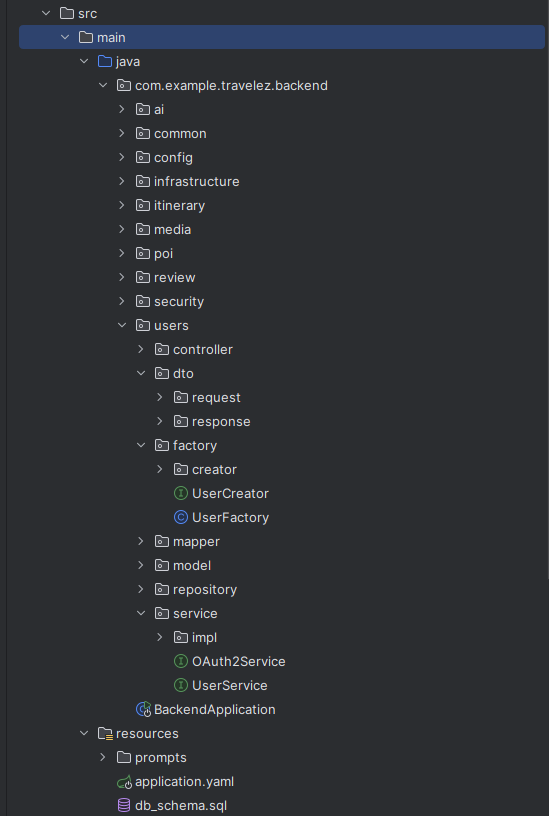
\includegraphics[width=0.8\textwidth]{Images/8. Implement/backend/backend_1.png}
    \caption{Cấu trúc thư mục Backend của TravelEZ}
    \label{fig:backend-folder-structure}
\end{figure}

\begin{itemize}
    \item \texttt{src/main/java/.../backend/}: Mã nguồn chính, được chia thành các modules nghiệp vụ.
    \begin{itemize}
        \item \texttt{controller/}: Chứa các REST controller, đóng vai trò là lớp giao tiếp với frontend.
        \item \texttt{dto/}: Chứa các đối tượng truyền tải dữ liệu, được phân chia rõ ràng để kiểm soát dữ liệu đầu vào/đầu ra:
        \begin{itemize}
            \item \texttt{request/}: Định nghĩa cấu trúc dữ liệu gửi lên từ Client.
            \item \texttt{response/}: Định nghĩa cấu trúc dữ liệu trả về cho Client.
        \end{itemize}
        \item \texttt{mapper/}: Chứa các Interface chịu trách nhiệm chuyển đổi dữ liệu giữa DTO và Entity. 
        \item \texttt{service/}: Chứa logic nghiệp vụ cốt lõi.
        \item \texttt{repository/}: Quản lý truy xuất dữ liệu với Spring Data JPA.
        \item \texttt{model/}: Các Entity ánh xạ trực tiếp với cơ sở dữ liệu.
    \end{itemize}
    \item Library toàn hệ thống:
    \begin{itemize}
        \item \texttt{infrastructure/}: Giao tiếp với các dịch vụ bên ngoài, giúp cô lập logic nghiệp vụ khỏi sự phụ thuộc vào các nhà cung cấp hạ tầng cụ thể.
        \item \texttt{ai/}: Module lõi xử lý các tác vụ thông minh, quản lý ngữ cảnh và tích hợp với các công cụ để thực hiện gợi ý hành trình.
        \item \texttt{common/}: Các thành phần dùng chung toàn hệ thống (BaseEntity, Global Exception Handler, Utils,...).
        \item \texttt{config/}: Cấu hình toàn cục (Spring Bean, Database) 
        \item \texttt{security/}: Cấu hình bảo mật (JWT Authentication, CORS).
    \end{itemize}
    \item \texttt{src/main/resources/}:
    \begin{itemize}
        \item \texttt{prompts/}: Chứa các kịch bản (Prompt Engineering templates) được tinh chỉnh cho AI.
        \item \texttt{application.yaml}: Cấu hình biến môi trường hệ thống.
        \item \texttt{db\_schema.sql}: Script khởi tạo cấu trúc cơ sở dữ liệu.
    \end{itemize}
\end{itemize}
Áp dụng Factory và Strategy Pattern trong module users:
\begin{itemize}
    \item \texttt{UserFactory}: Đóng vai trò Factory điều phối việc khởi tạo đối tượng.
    \item \texttt{UserCreator \& thư mục creator/}: Áp dụng Strategy Pattern để định nghĩa các chiến lược khởi tạo cho từng loại người dùng (Traveler, Provider, Admin). 
\end{itemize}
\begin{figure}[htp]
    \centering
    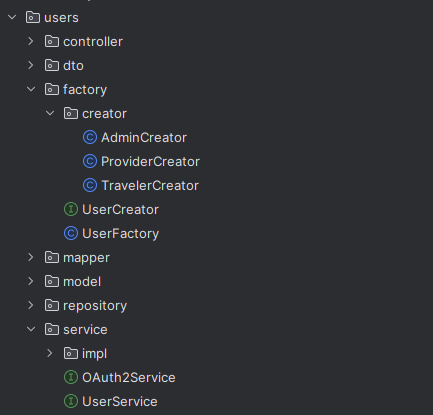
\includegraphics[width=0.8\textwidth]{Images/8. Implement/backend/backend_2.png}
    \caption{Áp dụng Factory và Strategy Pattern trong module users}
    \label{fig:factory-and-strategy-pattern}
\end{figure}

\subsubsection{Cách chạy dự án}
Mã nguồn backend được quản lý tại \url{https://github.com/TravelEZ-2025-2026/travelez-backend.git}

\begin{enumerate}
    \item Clone repository:
    \begin{verbatim}
git clone https://github.com/TravelEZ-2025-2026/travelez-backend.git
cd travelez-backend
    \end{verbatim}
    \item Thiết lập các biến môi trường trong trong hệ thống
    \begin{verbatim}
# Database
DB_URL=jdbc:postgresql://localhost:5435/travelez
DB_USERNAME=travelez
DB_PASSWORD=travelez

# Google cloud
GOOGLE_CLIENT_ID=your_google_client_id
GOOGLE_CLIENT_SECRET=your_google_client_secret
GOOGLE_REDIRECT_URI=http://localhost:3000/callback
RECAPTCHA_SECRET=your_recaptcha_secret

# JWT Authentication
SECRET_JWT=your_jwt_secret
JWT_EXPIRATION=604800

# Gemini AI
GEMINI_API_KEY=your_gemini_api_key
    \end{verbatim}
    \item Chạy ứng dụng backend
    \begin{verbatim}
mvn spring-boot:run
    \end{verbatim}
\end{enumerate}
